\documentclass{beamer}

\usepackage{xcolor}
\usepackage{booktabs}
\usepackage{graphicx}
\usepackage{algorithm, algpseudocode}
\usepackage{textpos}
\usepackage{verbatim}
%\usepackage{algorithm,algorithmic}

\setbeamertemplate{caption}[numbered]

\usepackage{tikz}
\usetikzlibrary{shapes.geometric}
\usetikzlibrary{arrows,shapes,trees}
\usetikzlibrary{calc,shapes.multipart,chains,arrows}

\usepackage{listings}
\lstset{language=Java,
    showspaces=false,
    showtabs=false,
    breaklines=true,
    showstringspaces=false,
    breakatwhitespace=true,
    commentstyle=\color{green},
    keywordstyle=\color{blue},
    stringstyle=\color{red},
    basicstyle=\footnotesize,
    moredelim=[is][\textcolor{grey}]{\%\%}{\%\%}
}

\definecolor{gray}{rgb}{0.4,0.4,0.4}
\definecolor{darkblue}{rgb}{0.0,0.0,0.6}
\definecolor{cyan}{rgb}{0.0,0.6,0.6}

\lstdefinelanguage{XML}{
    morestring=[b]",
    morestring=[s]{>}{<},
    morecomment=[s]{<?}{?>},
    stringstyle=\color{black},
    identifierstyle=\color{darkblue},
    keywordstyle=\color{cyan},
    morekeywords={xmlns,version,type}% list your attributes here
}

\usetheme{Madrid}
\useoutertheme{miniframes} % Alternatively: miniframes, infolines, split

% Setup the university's color pallette
\definecolor{UIUCorange}{RGB}{19, 41, 75} % UBC Blue (primary)
\definecolor{UIUCblue}{RGB}{232, 74, 39} % UBC Grey (secondary)

\setbeamercolor{palette primary}{bg=UIUCorange,fg=white}
\setbeamercolor{palette secondary}{bg=UIUCblue,fg=white}
\setbeamercolor{palette tertiary}{bg=UIUCblue,fg=white}
\setbeamercolor{palette quaternary}{bg=UIUCblue,fg=white}
\setbeamercolor{structure}{fg=UIUCorange} % itemize, enumerate, etc
\setbeamercolor{section in toc}{fg=UIUCblue} % TOC sections

\setbeamercolor{subsection in head/foot}{bg=UIUCorange,fg=UIUCblue}
\setbeamercolor{subsection in head/foot}{bg=UIUCorange,fg=UIUCblue}

\usepackage[utf8]{inputenc}

%Information to be included in the title page:
\title{\textbf{Introduction to Objects and Abstract Data Types in Java}}
%\author{\textbf{Author}}
%\institute[\textbf{UIUC}]{\textbf{University of Illinois Urbana-Champaign}}
\date{}

\setbeamertemplate{title page}[default][colsep=-4bp,rounded=true]
\addtobeamertemplate{title page}{\vspace{3\baselineskip}}{}
\addtobeamertemplate{title page}{
    \begin{textblock*}{\paperwidth}(-1.0em, -1.2em)
        
\includegraphics[width=\paperwidth, height=\paperheight]{imgs/uiuc.jpg}
    \end{textblock*} 
}{}


\begin{document}

\pgfdeclarelayer{background}
\pgfsetlayers{background,main}

\tikzstyle{vertex}=[circle,fill=black!25,minimum size=20pt,inner sep=0pt]
\tikzstyle{selected vertex} = [vertex, fill=orange!24]
\tikzstyle{edge} = [draw,thick,-]
\tikzstyle{weight} = [font=\small]
\tikzstyle{selected edge} = [draw,line width=5pt,-,blue!50]
\tikzstyle{ignored edge} = [draw,line width=5pt,-,black!20]


\frame{\titlepage}

\section{Objectives}
\begin{frame}
	\frametitle{Objectives}
    \centering
    \begin{itemize}
		\item Understand and be able to write basic Extensible Markup Language (XML)
        \item Understand how to parse XML in Java
        \item Construct objects using data parsed from XML
		\item Read user input in Java and use it to direct the control flow of a program
    \end{itemize}
\end{frame}


\section{XML and the DOM}
\begin{frame}
    \frametitle{XML and DOM}
    \begin{itemize}
        \item \textbf{XML: } Extensible Markup Language is a flexible language that allows us to store data in a hierarchical fashion.
        \item \textbf{DOM: } The Document Object Model is the hierarchical structure that is defined by an XML document.
        \item When we parse XML we are creating a DOM.
    \end{itemize}
\end{frame}

\begin{frame}[fragile]
    \frametitle{Basics of XML}
    \begin{itemize}
        \item We can create pairs of tags to encapsulate data:
            \begin{itemize}
                \item \lstinline|<name>Eluvetie</name>|
                \item \lstinline|<genre>Folk Metal</genre>|
            \end{itemize}
        \item We can group pairs of tags together with other tags:
        \begin{lstlisting}[basicstyle=\scriptsize, language=XML]
        <band>
            <name> Eluvetie </name>
            <genre> Folk Metal </genre>
        </band>
        \end{lstlisting}
    \end{itemize}
\end{frame}

\begin{frame}[fragile]
    \frametitle{Basics of XML}
    And we can keep growing these collections
    \begin{lstlisting}[basicstyle=\scriptsize, language=XML]
    <band>
        <name> Eluvetie </name>
        <genre> Folk Metal </genre>
        <songs>
            <songname> A Rose for Epona </songname>
            <songname> Omnos </songname>
            <songname> Lvgvs </songname>
        </songs
    </band>
    \end{lstlisting}
\end{frame}

% Key Point: XML lets us label and organize data 
\begin{frame}[fragile]
    \frametitle{Basics of XML}
    And we can keep growing these collections
    \begin{lstlisting}[basicstyle=\scriptsize, language=XML]
    <bands>
        <band>
            <name> Eluvetie </name>
            <genre> Folk Metal </genre>
            <songs>
                <songname> A Rose for Epona </songname>
                <songname> Omnos </songname>
                <songname> Lvgvs </songname>
            </songs
        </band>
        <band>
            <name> Slice the Cake </name>
            <genre> Prog. Metal </genre>
            <songs>
                <songname> Westward Bound - Part 1</songname>
                <songname> Westward Bound - Part 2</songname>
            </songs
        </band>
    </bands>
    \end{lstlisting}
\end{frame}

\section{Parsing XML in Java}
\begin{frame}
    \frametitle{The lay of the land}
    \begin{enumerate}
        \item Create an instance of the \lstinline|DocumentBuilderFactory| object.
        \item Use the \lstinline|DocumentBuilderFactor| to create a \lstinline|DocumentBuilder|. We will be using this object to parse our XML.
        \item Open the file by creating a new \lstinline|File| object.
        \item Use our document builder to parse the XML in the \lstinline|File| object.
    \end{enumerate}
\end{frame}

\begin{frame}[fragile]
    \frametitle{DocumentBuilderFactory}
    \begin{lstlisting}[basicstyle=\tiny]
    DocumentBuilderFactors dbf = DocumentBuilderFactory.newInstances()
    \end{lstlisting}
    \begin{itemize}
        \item A factory is a class that is responsible for making instances of other classes.
        \item Factories are a common design pattern in Object Oriented Programming.
        \item \lstinline|DocumentBuilderFactories| produces \lstinline|DocumentBuilder|
    \end{itemize}
\end{frame}

\begin{frame}[fragile]
    \frametitle{DocumentBuilder}
    \begin{lstlisting}[basicstyle=\tiny]
    DocumentBuilderFactors dbf = DocumentBuilderFactory.newInstances()

    DocumentBuilder db = null;
    try{
        db = dbf.newDocumentBuilder();
    } catch(ParserConfigurationException e){
        System.out.println("Failed to configure document builder object");
    }
    \end{lstlisting}
    \begin{itemize}
        \item We use our \lstinline|dbf| to instantiate a new \lstinline|DocumentBuilder| via the \lstinline|newDocumentBuilder()| method.
        \item Calling this function can produce an \lstinline|ParserConfigurationException| which Java requires us to catch.
    \end{itemize}
\end{frame}

\begin{frame}[fragile]
    \frametitle{File}
    \begin{lstlisting}[basicstyle=\tiny]
    DocumentBuilderFactors dbf = DocumentBuilderFactory.newInstances()

    DocumentBuilder db = null;
    try{
        db = dbf.newDocumentBuilder();
    } catch(ParserConfigurationException e){
        System.out.println("Failed to configure document builder object");
    }

    File f = new File(filePath)
    \end{lstlisting}
    \begin{itemize}
        \item Now that we have our XML parser which will build our DOM we need to open the file.
        \item We provide the \lstinline|File| class's constructor the path to our XML file.
    \end{itemize}
\end{frame}

\begin{frame}[fragile]
    \frametitle{Document}
    \begin{lstlisting}[basicstyle=\tiny]
    DocumentBuilderFactors dbf = DocumentBuilderFactory.newInstances()

    DocumentBuilder db = null;
    try{
        db = dbf.newDocumentBuilder();
    } catch(ParserConfigurationException e){
        System.out.println("Failed to configure document builder object");
    }

    File f = new File(filePath)

    Document doc = null;
    try{
        doc = db.parse(f);
    } catch(SAXException | IOEXception e){
        System.out.println("Failed to parse document.")
    }
    \end{lstlisting}
    \begin{itemize}
        \item Finally, we create our \lstinline|Document| (i.e., the DOM) by giving the document builder our opened file.
        \item There are two exceptions that can occur. Either the XML may not be valid or the file may not be readable. Java requires that we catch both of these.
    \end{itemize}
\end{frame}

\begin{frame}[fragile]
    \frametitle{Nodes}
    \begin{minipage}{0.35\textwidth}
        \begin{lstlisting}[basicstyle=\tiny, language=XML]
<bands>
  <band>
    <name> Eluvetie </name>
    <genre> Folk Metal </genre>
  </band>
  <band>
    <name> Slice the Cake </name>
    <genre> Prog. Metal </genre>
  </band>
</bands>
        \end{lstlisting}
    \end{minipage}
    \begin{minipage}{0.64\textwidth}
        \begin{itemize}
            \item The document produced ends up being a collection of Nodes
            \begin{itemize}
                \tiny
                \item A ``Node'' is all the XML between two tags.
            \end{itemize}
            \item We can get a list of nodes (NodeList) via: 
            \begin{itemize}
                \tiny
                \item NodeList nodes = doc.getElementsByTagName("tagName").
            \end{itemize}
            \item We can get an individual node from that node list via:
            \begin{itemize}
                \tiny
                \item Node node = nodes.item(i).
            \end{itemize}
            \item We can get the text content from the node via: 
            \begin{itemize}
                \tiny
                \item String nodeText = node.getTextContent().
            \end{itemize}
        \end{itemize}
    \end{minipage}
\end{frame}

\begin{frame}[fragile]
    \frametitle{Worksheet: XML Parsing}
    Off to the worksheet to see how this works in practice!
\end{frame}

\begin{frame}[fragile]
    \frametitle{Why Bother With XML?}
    \begin{minipage}{0.4\textwidth}
        \begin{lstlisting}[basicstyle=\tiny, language=XML]
<bands>
  <band>
    <name> Eluvetie </name>
    <genre> Folk Metal </genre>
  </band>
  <band>
    <name> Slice the Cake </name>
    <genre> Prog. Metal </genre>
  </band>
</bands>
        \end{lstlisting}
    \end{minipage}
    \begin{minipage}{0.59\textwidth}
        \begin{itemize}
            \item We often want to separate the program from the data it is using.
                \begin{itemize}
                    \item Imagine we wanted to make a music player app. 
                    \item App and songs the app plays are separate.
                \end{itemize}
            \item XML provides a structured and (relatively) easy to parse method of doing this.
            \item There are other methods of storing data:
            \begin{itemize}
                \item Comma Separated Values (csv) files
                \item Databases (e.g., SQL, SQLite, MongoDB)
            \end{itemize}
        \end{itemize}
    \end{minipage}
\end{frame}

\section{Instantiating Objects with XML Data}
\begin{frame}[fragile]
    \frametitle{We can read data. Now what?}
        Class 1: A class to store data/methods
        \begin{lstlisting}[basicstyle=\tiny]
class Bands{
    String name;
    String genre;
    Bands(String name, String genre){
        this.name = name;
        this.genre = genre;
    }
}
        \end{lstlisting}
        \vfill
        Class 2: A class to read data from the file
        \begin{lstlisting}[basicstyle=\tiny]
class ParseBands{
    public static void main(String[] args){
        // Parse all bands into NodeList called bands
        List<Bands> bandList = new ArrayList<>();
        for(int i = 0; i < bands.getLength(); i++){
            Element elem = (Element) bands.item(i); 

            String name = elem.getElementsByTagName("name").item(0).getTextContent();
            String genre = elem.getElementsByTagName("genre").item(0).getTextContent();

            bandList.add(new Bands(name, genre));
        }
    }
}
        \end{lstlisting}
\end{frame}

\begin{frame}[fragile]
    \frametitle{Worksheet: XML Parsing and Objects}
    Off to the worksheet to see how this works in practice!
\end{frame}

\section{User Input}
\begin{frame}[fragile]
    \frametitle{Getting Keyboard Input from the User}
    \begin{lstlisting}[basicstyle=\scriptsize]
Scanner sc = New Scanner(System.in);
System.out.print("Enter value: ")
    \end{lstlisting}
    \begin{itemize}
        \item \lstinline|System.in| is the standard input stream for your computer (a.k.a., keyboard).
        \begin{itemize}
            \item Others include \lstinline|System.err| and \lstinline|System.out|.
        \end{itemize}
        \item \lstinline|Scanner| ``watches'' that stream and waits for: 1) data and 2) a newline in order to determine that input has ended.
        \item Depending on what we want we can use the following functions to get a value from the \lstinline|Scanner|:
        \begin{itemize}
            \item \lstinline|Integer val = sc.nextInt()|
            \item \lstinline|Float val = sc.nextFloat()|
            \item \lstinline|String val = sc.nextLine()|
            \item \lstinline|Double val = sc.nextDouble()|
        \end{itemize}
    \end{itemize}
\end{frame}

\section{Putting it all Together}

\begin{frame}[fragile]
    \frametitle{Extending our Filtering Pattern}
    \begin{lstlisting}[basicstyle=\scriptsize]
class Animal implements Comparable<Animal>{
    //...
    @Override
    public int compareTo(Animal other){
        return name.compareTo(other.name);
    }
}
    \end{lstlisting}
    \vfill
    \begin{itemize}
        \item If we are going to build and potentially sort information we need some method of comparing two classes
        \item Our class must \lstinline|implement| the \lstinline|Comparable| interface
        \item We must also override the compareTo method of that interface.
            \begin{itemize}
                \item Generally involves calling the compareTo method of some attribute of the class.
            \end{itemize}
    \end{itemize}
\end{frame}

\begin{frame}
    \frametitle{XML Parsing + Making Objects + Filtering + User Input}
    \vfill
    \begin{figure}
        \centering
        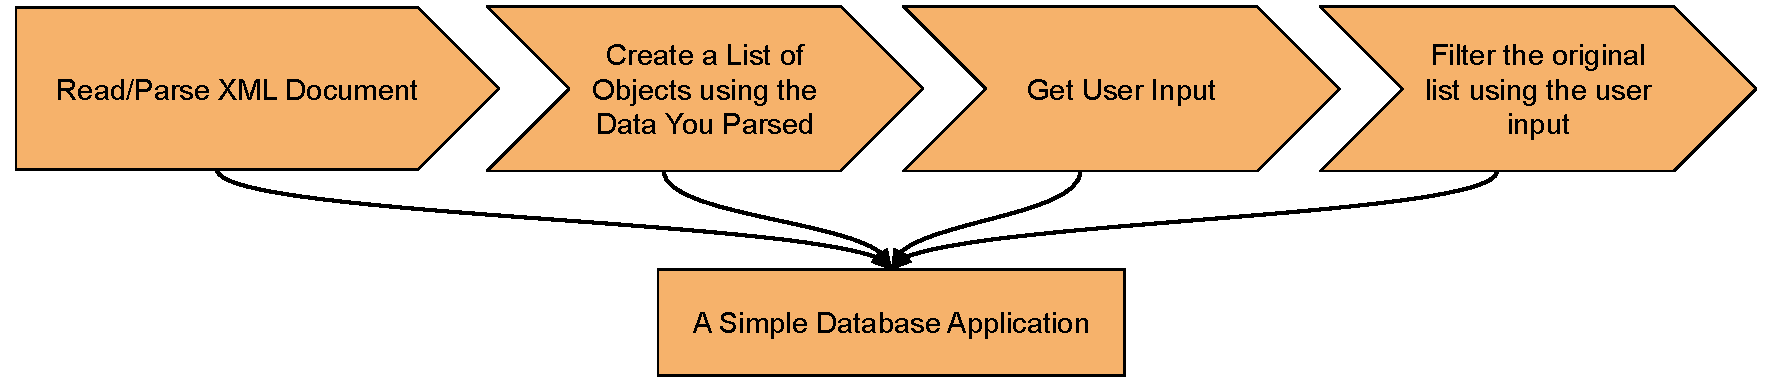
\includegraphics[width=\textwidth]{./imgs/databaseapp.pdf}
    \end{figure}
    \vfill
    Off to the worksheet to practice this!
\end{frame}

\end{document}
